\documentclass[TP, noCustomPackages]{UPSTI_Document}
\usepackage{listings}
\usepackage{lstautogobble}
\usepackage{hyperref}
\usepackage{fontawesome}
\usepackage{multirow}
\usepackage{multicol}
\usepackage{currfile}
\usepackage{pdfpages}
\usepackage{placeins}
%\usepackage{pdftricks}




% \begin{psinputs}
%     \usepackage{pstricks}
%     \usepackage{pstricks-add}
%     \usepackage{pst-eucl}
%     \usepackage{color}
%     \usepackage{pstcol}
%     \usepackage{pst-plot}
%     \usepackage{pst-tree}
%     \usepackage{pst-eps}
%     \usepackage{multido}
%     \usepackage{pst-node}
%     \usepackage{pst-eps}
% \end{psinputs}

\definecolor{vert}{rgb}{0.0, 0.5, 0.0}

\newlength{\iconeHeight}
\setlength{\iconeHeight}{15pt}

\newcommand{\UPSTIvariante}{2}


\newlist{todolist}{itemize}{2}
\setlist[todolist]{label=$\square$}
\newcommand{\UPSTIclasse}{S1}
\discipline[Autom - Robotique]{Automatisme pour la robotique}
\edef\CurrentFileDir{\currfiledir} 
\graphicspath{{\CurrentFileDir figures/}}



\newcommand{\basepath}{U:\textbackslashDocuments\textbackslashBUT\textbackslashGEII\textbackslashModulesS5\textbackslashAutomatisme_Pour_Robotique\textbackslash}
\newcommand{\subdir}[1]{\basepath{}#1}


%%% Définition du langage ST %%%
%New colors defined below
\definecolor{codegreen}{rgb}{0,0.6,0}
\definecolor{codegray}{rgb}{0.5,0.5,0.5}
\definecolor{codepurple}{rgb}{0.502,0.502,0.0}
\definecolor{backcolour}{rgb}{0.95,0.95,0.95}

\lstdefinelanguage{ST}
{
	morekeywords={
	case,of,if,then,end_if,end_case,super,function_block,extends,var,
	constant, byte,,end_var,var_input, real,bool,var_output,
	dint,udint,word,dword,array, of,uint,not,adr, program, for, end_for, while, do, end_while, repeat, end_repeat, until, to, by, else, elsif, var_in_out,interface,method,property
	},
	otherkeywords={
		:, :=, <>,;,\,.,\[,\],\^,1,2,3,4,5,6,7,8,9,0,TRUE, FALSE, \{attribute,  \'hide\'\}
	},
	keywords=[1]{
		case,of,if,then,end_if,end_case,super,function_block,extends,var,
		constant, byte,,end_var,var_input, real,bool,var_output,
		dint,udint,word,dword,array, of,uint,not,adr, :, :=, <>,;,\,.,\[,\],\^,program, for, end_for, while, do, end_while, repeat, end_repeat, until, to, by, else, elsif, var_in_out,interface,method,property
	},
	keywordstyle=[1]\color{blue},
	keywords=[2]{
		1,2,3,4,5,6,7,8,9,0, TRUE, FALSE
	},
	keywordstyle=[2]\color{codepurple},
	keywords=[3]{
		\{attribute,  \'hide\'\}
	},
	keywordstyle=[3]\color{codegray},
	sensitive=false,
	morecomment=[l]{//}, 
	morecomment=[s]{(*}{*)},
	morestring=[b]{"},
	morestring=[b]{'}
}

\lstset{
	language={ST},
	backgroundcolor=\color{backcolour},
	commentstyle=\color{codegreen}\textit,
	keywordstyle=\color{blue},
	numberstyle=\tiny\color{codegray},
	stringstyle=\color{codepurple},
	basicstyle=\ttfamily\scriptsize,
	breakatwhitespace=false,         
	breaklines=true,                 
	captionpos=b,                    
	keepspaces=true,                 
	numbers=left,                    
	numbersep=5pt,                  
	showspaces=false,                
	showstringspaces=false,
	showtabs=false,                  
	tabsize=2
}
%\lstMakeShortInline[columns=fixed]~
\newcommand{\UPSTItitreEnTete}{Informatique industrielle}
\newcommand{\UPSTItitre}{Conversions Analogique-Numérique}


\newcommand{\UPSTItitre}{Détournement d'un téléphone à clavier}

\documentVersion{E}
\newcommand{\UPSTInumeroVersion}{1}
\begin{document}
\begin{figure}[h!bt]
    \centering
    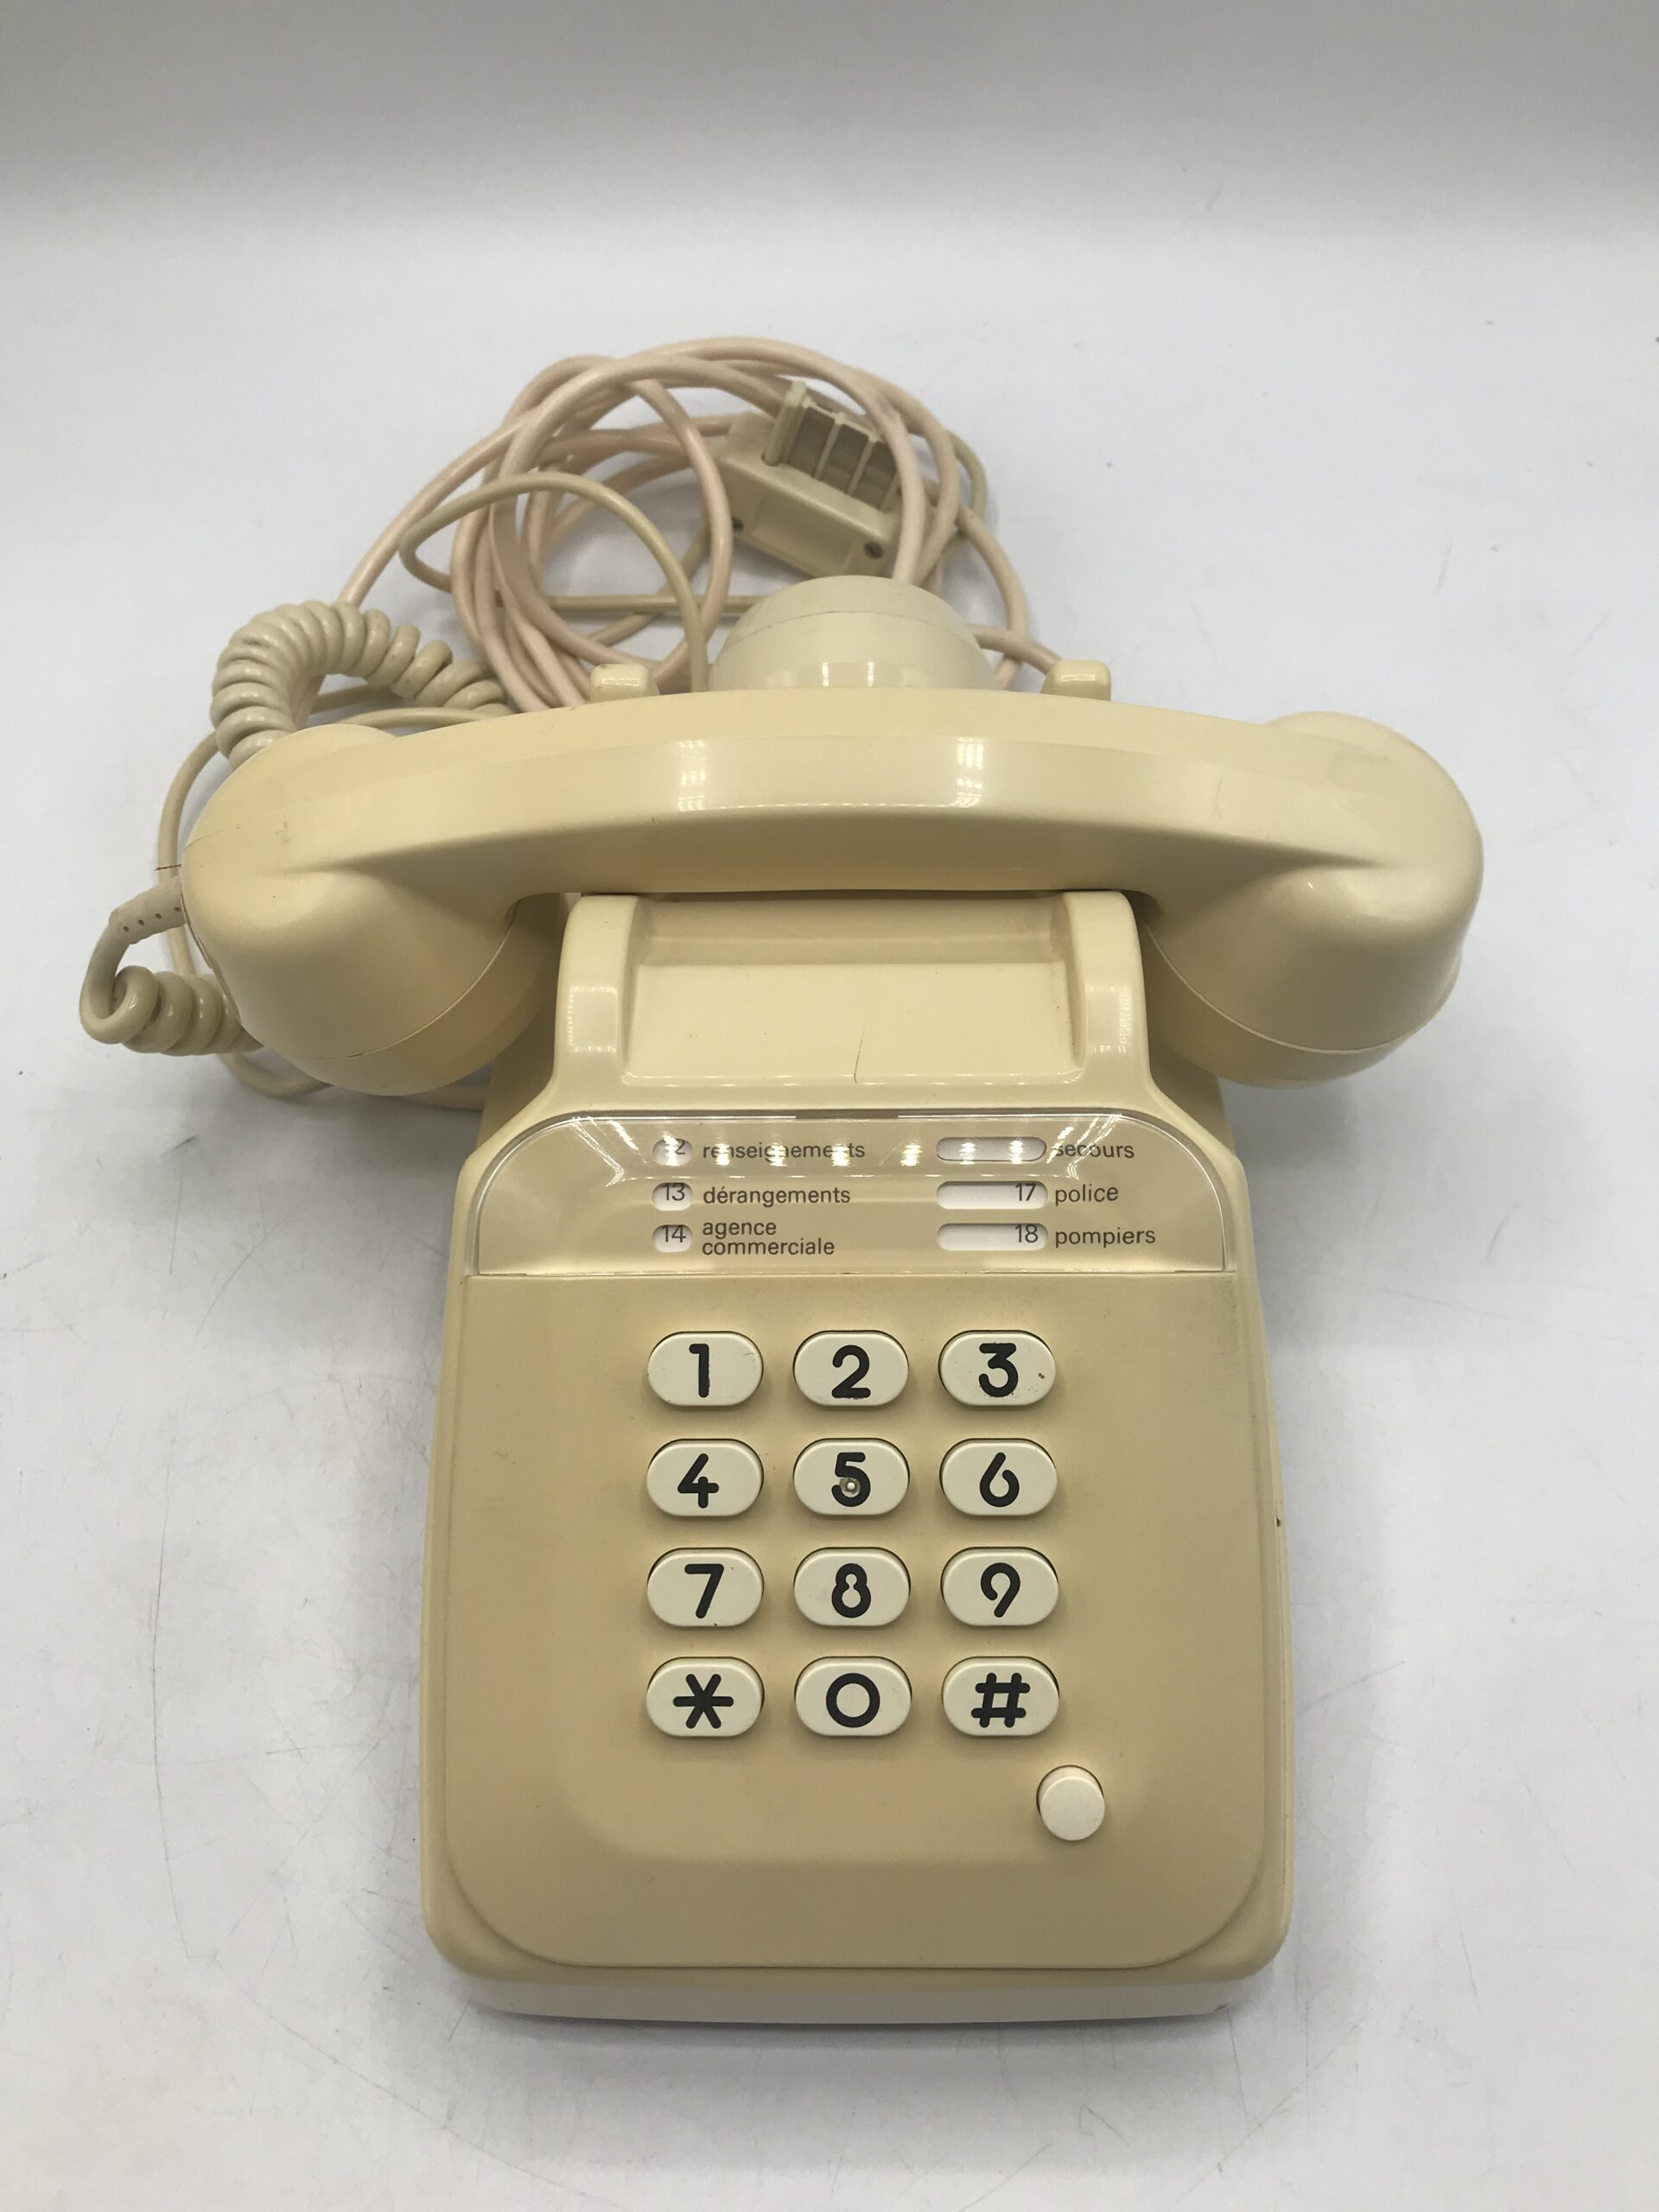
\includegraphics[width=.4\textwidth, trim= 0mm 10mm 0mm 100mm, clip]{images/telephone-Socotel-S63.jpg}
    \caption{Socotel S63}
\end{figure}


Matériel à disposition : 
\begin{itemize}
    \item Un téléphone ancien à clavier. 
\end{itemize}

\begin{UPSTIactivite}[2][Composition d'un numéro de téléphone][][][Cahier des charges]
    L'utilisateur doit pouvoir composer un numéro de téléphone en sur le clavier. Le numéro composé s'affichera sur le terminal de la liaison série. Au bout de 10 chiffres ou si le téléphone est raccroché, une nouvelle ligne permettra de composer un nouveau numéro.

    Si le téléphone est raccroché, le clavier ne doit pas être pris en compte.
\end{UPSTIactivite}

\begin{UPSTIactivite}[2][Faire sonner le téléphone][][][Cahier des charges]
    Lorsque le téléphone est raccroché, la composition d'un chiffre doit faire sonner le téléphone un nombre de fois égal à la valeur du chiffre composé.
    Chaque sonnerie doit durer 1 seconde et être séparée de la suivante par une pause de 1 seconde.
\end{UPSTIactivite}

\begin{UPSTIactivite}[4][Audio][][][Cahier des charges]
    Lorsque le téléphone est décroché, l'utilisateur doit pouvoir entendre un son de fréquence \SI{440}{Hz} tant qu'il n'a pas composé de numéro.
    Une fois un numéro complet composé, le téléphone doit émettre un son de fréquence \SI{440}{Hz} pendant 1 seconde puis un message vocal doit être diffusé.
\end{UPSTIactivite}

\begin{UPSTIactivite}[4][ Enregistrement][][][Cahier des charges]
    Cahier des charges 3 + Enregistrement d'un message. 
\end{UPSTIactivite}

\end{document}